\newpage
\section{Mögliche Aspekte}
\subsection{Persönliche mobile Arbeitsumgebung}
\subsubsection{Funktionalität}
Heutzutage werden Computer für alle möglichen Tätigkeiten in der Arbeitswelt benötigt, ob nun für kleinere Aufgaben oder für komplexe Berechnung mit Hilfe eines am Netzwerk angeschlossenen Supercomputers. In einer modernen Umgebung kann es unter Umständen notwendig sein den Arbeitsplatz aufgrund einer Tätigkeit zu wechseln um diese ausführen zu können. Dies hat allerdings zur Folge, dass dort der eigene Rechner mit den zugehörigen Daten und möglicherweise auch die benötigte Rechenleistung nicht verfügbar ist.
Um für die Benutzer eine auf allen Rechnersystemen einheitliche Bedienerfahrung gewährleisten zu können, lässt sich eine sogenannte mobile personalisierte virtuelle Computerumgebung (MOVE)\nomenclature{MOVE}{Mobile Personalized Virtual Computing Environment} nutzen. Durch diese Umgebung wird dem Benutzer auf jeder beliebigen Maschine eine gleichmäßig konsistente Desktop-Rechner-Umgebung präsentiert, welche sowohl die gleichen personenbezogenen Daten und Software als auch die verfügbare Rechenleistung liefert wie am eigenen Arbeitsplatzrechner. Eine solche Desktop-Rechner-Umgebung besteht zum Großteil aus der installierten Software einschließlich des Betriebs- und Dateisystems. Diese könnten zwar vom Speichermedium auf ein anderes übertragen werden, aufgrund der engen Koppelung ließe sich diese allerdings nicht einfach auf einem neuen System ausführen. Um diese Abstraktion gewährleisten zu können, wird die Technologie der virtuellen Maschinen (VM)\nomenclature{VM}{Virtual Maschine} genutzt.\footcite[Vgl.][Seite 890 f.]{MOVE}

Bei der Virtualisierung werden mit Hilfe von Technologien die Ressourcen eines Rechnersystems auf mehrere einzelne Klienten aufgeteilt um diese effektiver und flexibler nutzbar zu machen. Dies geschieht dadurch, dass unterschiedliche Klassen von Anwendungen auf wenigen physischen Systemen konsolidiert und von mehreren unabhängigen Betriebssysteminstanzen gleichzeitig genutzt werden können.\footcite[Vgl.][Seite 197]{InformatikSpektrum} Diese Virtualisierung wird mit der Hypervisor Technologie implementiert. Ein Hypervisor, oder auch Virtual Maschine Monitor (VMM)\nomenclature{VMM}{Virtual Maschine Monitor} genannt, ist ein Stück Hardware oder Software welches Systemressourcen virtualisiert, wobei zwischen Typ 1 und Typ 2 Hypervisors unterschieden wird. Typ 1 Hypervisors sind direkt auf der Hardware implementiert, Typ 2 Hypervisors laufen dagegen auf einem Host Betriebssystem. Dieses stellt Dienste wie Speichermanagement zur Virtualisierung zur Verfügung.\footcite[Vgl.][]{ibm}

\begin{figure}[H]
\begin{center}
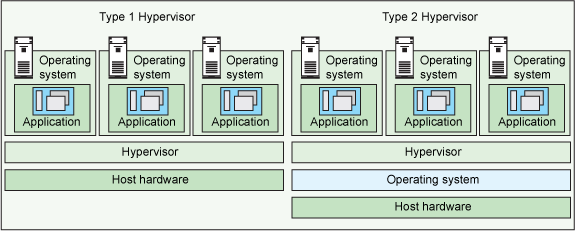
\includegraphics[width=0.9\textwidth]{hypervisors}
\caption{Unterschiede zwischen den Typ 1 und Typ 2 Hypervisors}
Quelle: \cite[]{ibm}
\end{center}
\end{figure}
\vspace{-1cm}

Solch ein zwischen Host-Hardware-Maschine und Gastsoftware implementierter VMM ermöglicht in diesem Fall die Koexistenz mehrerer Gastbetriebssysteme auf einer einzigen Single-Host-Hardwareplattform, indem eine vollständige Abstraktion von virtualisierten Hardwareressourcen zur Verfügung gestellt wird. Die Gastbetriebssysteme sind voneinander isoliert und können, entkoppelt und unabhängig von der zugrunde liegenden Hardware, auf dieser virtualisierten Plattform arbeiten. Die einzige Voraussetzung zur unmodifizierten Ausführung des Betriebssystems auf dem neuen Computer ist die Bereitstellung der gleichen virtuellen Plattform auf dem Zielsystem. Die Daten einer Computing-Umgebung lassen sich zusätzlich aufgrund der Speicherung des Dateisystems und des Software-Stacks beispielsweise als Image-Datei sehr einfach auf ein anderes System übertragen. Dies bedeutet, dass der VMM auf jedem davon unterstützten Gerät als eine einheitliche virtuelle Betriebssystemplattform dienen kann.\footcite[Vgl.][Seite 891]{MOVE}

\subsubsection{Aufbau eines MOVE Systems}
Ein MOVE System besteht im Großen und Ganzen aus vier Komponenten: einem MOVE Client, einem MOVE Server, privaten Netzwerkressourcen und einem IP Netzwerk. Das firmeninterne private LAN wird gebildet durch den MOVE Server und den übrigen privaten Netzwerkressourcen, der MOVE Client hingegen kann jede beliebige Maschine im Netzwerk sein und ist über das IP Netz mit dem privaten LAN verbunden. 
Der Nutzer zieht sich an einem beliebigen MOVE Client über das Netz eine lauffähige Instanz seiner eigenen Computing-Umgebung. Diese Instanz ist die persönliche virtuelle Computing-Umgebung. Die Daten des Benutzers werden durch seine Aktivitäten manipuliert, weswegen zur Erhaltung einer einheitlichen Umgebung auf allen Clients jede Operation zur Manipulation ebenfalls direkt auf dem MOVE Server ausgeführt werden muss. Dadurch wird gewährleistet, dass zu jeder Zeit an jedem Client der Benutzer die gleiche Umgebung erhält, die er zuvor verlassen hat.\footcite[Vgl.][Seite 891 f.]{MOVE}

\begin{figure}[H]
\begin{center}
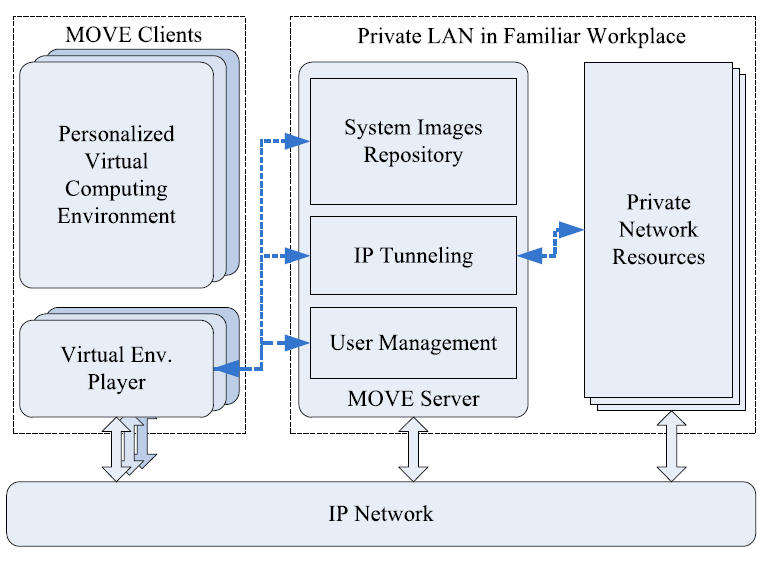
\includegraphics[width=0.9\textwidth]{move}
\caption{Komponenten einer MOVE Architektur}
Quelle: \cite[Seite 891]{MOVE}
\end{center}
\end{figure}
\vspace{-1cm}

Um diese Funktionalität zu ermöglichen sind einige Voraussetzungen notwendig. Zum einen wird für die Ausführung des persönlichen Desktops auf einem Client ein sogenanntes System Image benötigt. Dieses enthält alle Daten eines Nutzers, einschließlich des Betriebssystem, den Anwendungen und den persönlichen Dateien.
Daher werden alle System Images in Form von Image Dateien abgelegt, entweder als 
Festplattenimage oder als Partitionsimage und werden zentral im System-Image-Repository des MOVE Servers verwaltet. Dieses bietet zugleich die Funktionalität, einzelne Images aus dem Repository über das Netzwerk auf einen Client zu übertragen und gleichzeitig von diesen aus zu aktualisieren. Zum Anderen wird ein Virtual Environment Player benötigt, welcher einen auf einem tragbaren Speichermedium gelagerten Software-Stack darstellt. Wird ein physischer Computer gebootet, wird von dem angeschlossenen Speichermedium der Virtual Environment Player als virtuelle Plattform gestartet, wobei der VMM als Herzstück dient. Er kommuniziert zum Holen oder Aktualisieren des System Images mit dem System-Image-Repository des MOVE Servers und bietet eine Benutzerschnittstelle zur Auswahl des gewünschten Images. Zusätzlich wird eine Schnittstelle für den Zugriff auf die lokalen Dateien des Rechners bereitgestellt.\footcite[Vgl.][Seite 892]{MOVE}

Da jeder Benutzer nicht nur eine Computing-Umgebung und entsprechend nur ein System Image im Repository des MOVE Servers hinterlegt hat, ist eine Benutzererwaltung im System-Image-Repository erforderlich. Dieses bietet die Funktion für jeden Benutzer ein Profil anzulegen, in welchem sich dessen System Images pflegen lassen. Außerdem prüft es ob er ein für den Zugriff auf das private LAN berechtigter Benutzer ist. Weiterhin sind Ressourcen des lokalen privaten Netzwerks wie Hochleistungsrechner oder zentrale Fileserver Teil der MOVE Architektur. Unter Umständen kann es vorkommen, dass der Zugriff auf diese Ressourcen auf bestimmte Bereiche oder Subnetze des Unternehmens beschränkt ist, was die mobile Arbeit an jedem beliebigen Client unmöglich macht. Um diese Standortrestriktion zu umgehen wird daher die Technologie des IP Tunneling genutzt, welche zwischen den Virtual Environment Player und den MOVE Server geschaltet ist. Hierdurch wird die Kommunikation der beiden Komponenten über ein IP Tunneling Protokoll vollzogen und ermöglicht gleichzeitig dem MOVE Server die privaten Ressourcen für das externe Netzwerk freizugeben.\footcite[Vgl.][Seite 892]{MOVE}

\subsection{CGLXTouch}
\subsubsection{Problemstellung}
Multi-User-Kooperationsforschungsumgebungen bieten mit der richtigen Einbindung der Nutzer eine Vielzahl an Möglichkeiten im Arbeitsumfeld, vor allem in der wissenschaftlichen Erforschung und Analyse. Aufgrund der stetig wachsenden Gruppengrößen stellt deren Implementierung allerdings eine Herausforderung für Standardschnittstellenmodalitäten dar. Ansätze hierfür wurden bereits mit skalierbaren Displayumgebungen gemacht, bei denen aufgrund ihrer ultrahochauflösenden Auflösung mehrere Benutzer zeitgleich deren Inhalt betrachten können. Diese weisen aber noch einige Komplikationen auf. Zum einen besteht die Standardschnittstelle für die Bedienung dieser Geräte aus Maus und Tastatur, welche für den Single User Betrieb gedacht sind und keine Benutzung durch mehrere Benutzer gleichzeitig ermöglich. Zum anderen schränken Maus und Tastatur aufgrund ihrer stationären Bedienung beziehungsweise fehlender Mobilität die Nutzungsmöglichkeit der Geräte im Bezug auf die räumliche Ausdehnung ein. Speziell entwickelte Mehrbenutzerschnittstellen für die Steuerung der ultrahochauflösenden Bildschirme erfordern durch ihre Werkzeuge erweitertes Know-How und lassen sich zumeist nicht auf eine große Anzahl von Nutzern skalieren. Durch die technologischen Errungenschaften der letzten Jahre besitzt nun die Mehrheit der Arbeiter Multi-Touch-fähige Geräte mit vertrauten Bedienelementen, die zugleich eine nutzbare Schnittstelle zur Interaktion mit den genannten Systemen darstellen.\footcite[Vgl.][Seite 649]{Table}

\subsubsection{Funktionalität}
Aufbauend auf diesen technologischen Fortschritten bietet das folgende System einen Mehrbenutzerbetrieb für digitale Arbeitsplätze, sowohl durch herkömmliche Bedienelemente als auch durch Multi-Touch-Geräte. Hierdurch ist es Nutzern möglich, auf ultrahochauflösenden verteilten Displayumgebungen zeitgleich und gemeinsam zu arbeiten, wobei die einzelnen Displays als geteilte Leinwand dienen. Zur Interaktion dienen dabei zwei Technologien, zum einen die tragbaren Multi-Touch-Geräte der Benutzer auf denen visuelle Daten gestreamt werden und zum anderen nativ gerenderte Multi-Touch-Tischsysteme. Dadurch lassen sich komplexe Datenstrukturen auf einer Vielzahl von Geräten analysieren, welche einzeln bei Bedarf zum System hinzugefügt oder aus dem System entfernt werden können. Durch die zusätzliche Identifizierbarkeit der einzelnen Personen durch ihre respektiven Geräte ist der Grundstein für skalierbare Multi-Touch- und Mehrbenutzer-Arbeitsplätze gelegt.\footcite[Vgl.][Seite 649]{Table}

\subsubsection{Aufbau}
Das System besteht im Groben aus einem zentralen Head Node auf dem ein Device Manager implementiert ist, einer ultrahochauflösenden Leinwand mit einem oder mehreren Render Nodes, aktiven oder passiven Servern und der Cross-
Platform Cluster Graphic Library (CGLX)\nomenclature{CGLX}{Cross-
Platform Cluster Graphic Library} als Middleware (siehe Abbildung 3).\footcite[Vgl.][Seite 651 f.]{Table}

\begin{figure}[H]
\begin{center}
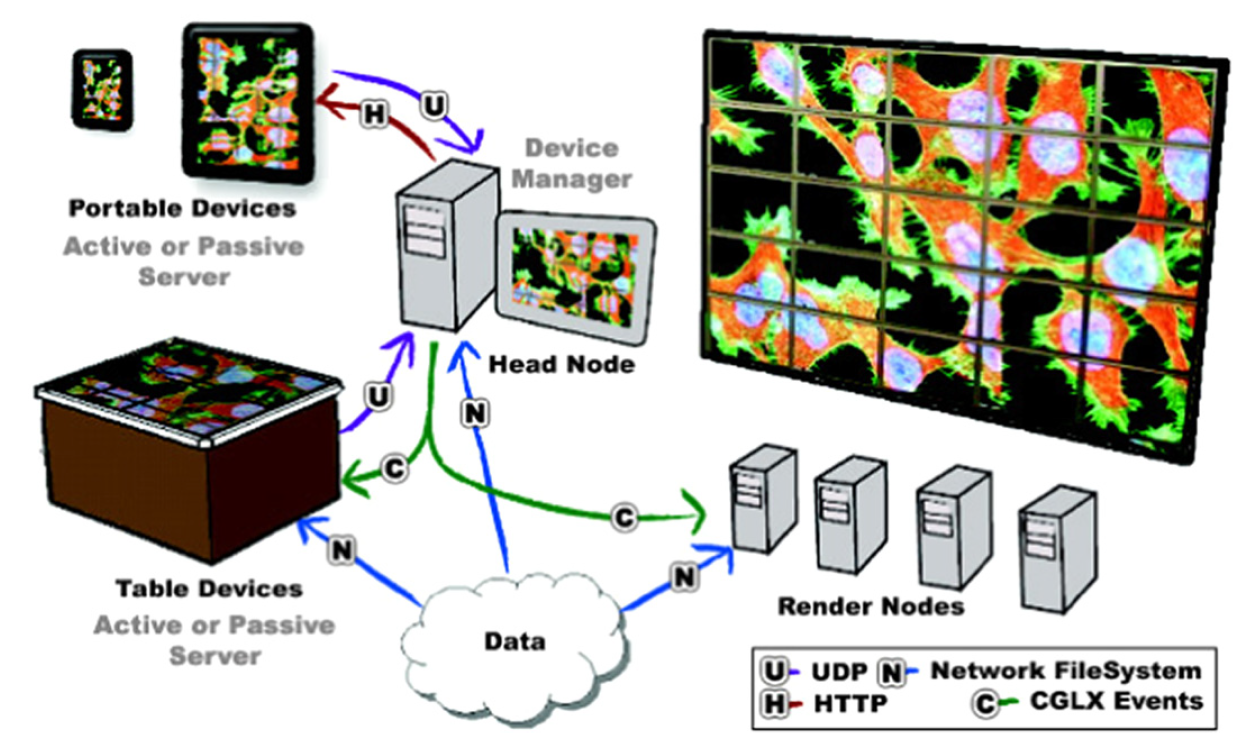
\includegraphics[width=0.9\textwidth]{table}
\caption{Aufbau der Systemarchitektur}
Quelle: \cite[Seite 651]{Table}
\end{center}
\end{figure}
\vspace{-1cm}

Die CGLX ist ein OpenGL-basiertes Grafik-Framework für verteilte Visualisierungssysteme. Sie ermöglicht es OpenGL-basierten Anwendungen, Visualisierungscluster wie hochauflösende verteilte Display-Umgebungen zu nutzen und die erreichbare Leistung und Auflösung zu maximieren.\footcite[Vgl.][Seite 320]{CGLX} Diese Technologie wird verwendet, um der Anforderung für das hochauflösende Rendern und Darstellen gerecht zu werden. Sie synchronisiert mithilfe von Mechanismen die Aktionen der Benutzer wie beispielsweise Eingaben über Maus und Tastatur und bestimmt die notwendigen Transformations- und Projektionsmatrizen zur Schaffung einer einheitlichen Anzeigeumgebung, an welche die Aktionen anschließend effizient weitergeleitet werden. Die Multi-Touch-Geräte der Benutzer kommunizieren über UDP direkt mit dem Head Node um die notwendige Leistungsanforderung zu erfüllen, auch unter dem Risiko des Datenverlustes bei der Transportation. Von dort aus werden die Daten durch die CGLX an die Anzeigeumgebung verteilt.\footcite[Vgl.][Seite 651]{Table}

Der Device Manager, welcher auf dem Head Node läuft, bietet die Unterstützung mehrerer gleichzeitig angeschlossener Geräte. Er wurde als neue Schicht mit der Zuständigkeit für die Organisation von und den Verbindungsaufbau zu den Geräte-Servern implementiert. Die von diesen Geräten ankommenden Aktionen werden vom Device Manager entgegengenommen, gesammelt und an das System weitergeleitet. Verbundene Geräte werden als aktiv betrachtet und in einer Server-Pool-Datenstruktur verwaltet, wobei hier zwischen aktiven und passiven Servern unterschieden wird.\footcite[Vgl.][Seite 651]{Table}

Passive Server sind für Geräte gedacht die standardmäßig angeschlossen und genutzt werden. Es muss hierbei keine Verbindung durch den Benutzer aufgebaut werden, da der Head Node während des Betriebs zyklisch prüft ob die passiven Server aktiv sind und den Verbindungsaufbau selbstständig anstößt. Der Device-Manager liest hierbei die hinterlegte Konfigurationsdatei ein, in welcher alle Passivserver definiert sind, und versucht anschließend alle dort aufgeführten Server zu aktivieren. Die hinterlegten Passivserver erhalten zu der Aktivierungsanforderung vom Geräte-Manager zusätzlich einen Servertyp, eine eindeutige ID und einen Kommunikationsport. Stimmt der Servertyp mit dem eigenen überein, werden die ID und der Kommunikationsport übernommen und gesetzt. Ist der Server erstmal zum Active-Server-Pool hinzugefügt worden, erhält er die Berechtigung Daten an den Head Node zu senden.
Aktive Server sind dagegen für Geräte gedacht, die nur sporadisch genutzt werden und ab und zu on-the-fly an eine laufende CGLX-Anwendung angeschlossen werden sollen. Es ist nicht notwendig diese in der XML-Konfigurationsdatei zu definieren, müssen im Gegenzug allerdings bei Start einer neuen Anwendung verbunden werden. Des Weiteren benötigen die aktiven Server die IP-Adresse des Head Nodes um eine Verbindungsanfrage senden zu können. Der darauf liegende Geräte-Manager empfängt diese und sendet bei einer erfolgreichen Prüfung ID und Kommunikationsport zurück an den Server. Identisch zum passiven Server werden auch die aktiven dem Server-Pool hinzugefügt und erhalten anschließend die Berechtigung zum Senden von Daten.\footcite[Vgl.][Seite 651 f.]{Table}

\subsubsection{Voraussetzungen}
Um diese Systemarchitektur zu betreiben, sind die oben genannten Komponenten erforderlich. Die passiven und aktiven Server sind zwar für die Funktion nicht zwingend notwendig, allerdings gäbe es ohne diese keinen Bedarf für solch ein System. Die hierfür nutzbaren Multi-Touch-Geräte sind weitreichend, von stationären Tischsystemen bis hin zu Allerlei tragbaren Geräten.

Der Vorteil von Touch-Table-Systemen ist die Möglichkeit, diese aufgrund ihrer stationären Aufstellung mit leistungsstarker Ausstattung zu versehen um so natives Rendering zu ermöglichen. Die Anbindung an das lokale Netzwerk erlaubt außerdem einen Zugriff auf weitere Netzwerkkomponenten und -laufwerke. Das hinter dem Berührungsdisplay zugrunde liegende System kann dadurch sogar als Head Node oder auch als weiterer Render Node in die Architektur eingebunden werden. 
Durch die Nutzung von tragbaren Multi-Touch-Geräten wie Mobiltelefonen und Tablets ist es den Nutzern möglich, sich frei im Raum zu bewegen. Für diese Apparate ist der Ansatz für aktive Server gedacht, durch welchen sie sich mit dem Betreten des Raumes mit dem System verbinden können und somit eine interaktive und simple Interaktion geboten wird.\footcite[Vgl.][Seite 652]{Table}

Tragbare Geräte bergen allerdings einige Probleme. Zum einen besitzen die meisten von ihnen nicht die Rechenkapazität oder einen Zugriff zu den notwendigen Daten, um den Inhalt wie ein Touch-Table-System nativ zu rendern. Zum anderen müssten zu entwickelnde Anwendungen sowohl auf tragbaren Geräten als auch auf geteilten Displayumgebungen gleichermaßen laufen, was sich meist als überaus kompliziert gestaltet. Nutzer aüßerten sich allerdings in ersten Anwenderstudien positiv über die Relevanz von direktem visuellen Feedback zu deren Aktionen. Da Vorschauauflösungen des geteilten Anzeigesystems durch den Head Node wiedergegeben werden können, ist dieser auch in der Lage Bilddaten zurück zu den tragbaren Geräten zu streamen. Dies geschieht indem zunächst jeder Frame auf dem Head Node gerendert wird, anschließend der Inhalt des Frontpuffers von der Grafikkarte zurückgelesen, codiert und an die registrierten Mobilgeräte über die Netzwerkschnittstelle gesendet wird.
Zum Versenden wird Rohpixelstreaming über eine UDP-Kommunikation verwendet. Der Vorteil ist hierbei die Geschwindigkeit der Datenübertragung und das Streamen der Daten über einen einzelnen Stream parallel an mehrere Geräte durch Multicast Kommunikation. Aufgrund von Breitbandanforderungen und den benötigten Transportmechanismen ist diese Methode nicht verlässlich bei der Nutzung von öffentlichen Netzen. Daher wird auf dem Head Node ein leichtgewichtiger HTTP-Server implementiert, über den sich die einzelnen Geräte verbinden können. Darüber hinaus werden die einzelnen Bilder in JPEG-Bilddateien umgewandelt um deren Größe vor der Übertragung zu verringern und anschließend in festgelegten Zeitabständen an die tragbaren Geräte versendet. Hierdurch lassen sich vom Head Node bis zu 10 Frames pro Sekunde an die mobilen Geräte übertragen.\footcite[Vgl.][Seite 652 f.]{Table}

In einer Smart Workplace Umgebung lässt sich diese Systemarchitektur in Meetingräumen implementieren. Mitarbeiter können sich durch ihre Smartphones frei mit dem System verbinden und gemeinsam in dem Meeting mitwirken. Da heutzutage jeder mindestens eines solcher tragbaren Multi-Touch-Geräte jederzeit mit sich trägt, lassen sich Meetings dadurch effektiv und interaktiver gestalten.